\documentclass[conference]{IEEEtran}

\usepackage{graphicx,times,amsmath,url}
\usepackage{fancyvrb}

\usepackage[numbers]{natbib}
%\bibpunct{(}{)}{;}{a}{}{,}

% possible keywords:
%   knowledge representation (general/other)
%   computer games
%   logic programming
%   general game playing
%   search in games

% To create the author's affliation portion using \thanks
\IEEEoverridecommandlockouts

\textwidth 178mm
\textheight 239mm
\oddsidemargin -7mm
\evensidemargin -7mm
\topmargin -6mm
\columnsep 5mm

\pdfinfo{
/Title (Ludocore: A Logical Game Engine for Modeling Videogames)
/Subject (IEEE CIG 2010)
/Author (Adam M. Smith, Mark J. Nelson, and Michael Mateas)}

\newcommand{\ludocore}{\textsc{ludocore}}
\newcommand{\Ludocore}{\textsc{Ludocore}}
\newcommand{\snippet}[1]{{\vspace{-0.4cm}\begin{align*}#1\end{align*}\vspace{-0.4cm}}}
\newcommand{\logical}[1]{$#1$}

\begin{document}

\title{\ \\ \LARGE\bf\textsc{Ludocore}: A Logical Game Engine for Modeling
Videogames\thanks{The authors are with the Expressive Intelligence Studio at
the University of California, Santa Cruz (email: amsmith@soe.ucsc.edu,
\mbox{mnelson@cc.gatech.edu}, michaelm@soe.ucsc.edu).}}

\author{Adam M. Smith, Mark J. Nelson, and Michael Mateas}

\maketitle
\begin{abstract}

\Ludocore{} is a logical ``game engine'', linking game rules as reasoned about by
game designers to the formal logic used by automated reasoning tools in AI.
A key challenge in designing this bridge is engineering a concise, safe, and
flexible representation that is compatible with the semantics of the games that
logical models created with our engine intend to represent.

Building on the event calculus, a formalism for reasoning about state and
events over time, and a set of common structures and idioms used in
modeling games, we present a tool that is capable of generating gameplay traces
that illustrate the game's dynamic behavior. It supports incremental modeling
of player and non-player entities in the game world, modification of game
rules without extensive non-local changes, and exploratory temporal and
structural queries. In addition, its logical models can support play as
real-time, graphical games with minimal user-interface description.

\end{abstract}

\section{Introduction}

While the term \emph{videogame} brings to mind graphics, sounds, and story
worlds, at the core of every game is a formal rule system. We are interested in
declaratively modeling these games so that the emergent properties of their
rule systems can be understood. The tools of logicist AI hold promise for
bringing such properties to light, but have not been used for design or
analysis of videogames, in part because of a mismatch between how designers
think of their rule systems and the way logical specifications are usually
written. We propose the use of a logical ``game engine'' to ease and accelerate
the modeling of game worlds in formal logic. Our engine, \ludocore, provides a
set of primitives and abstractions that link game-level concepts to the
first-order logic understood by AI reasoning tools. Specifically, our engine
supports automatically generating gameplay traces, integrated player modeling,
and both temporal and structural queries. Finally, games modeled in \ludocore{}
can be directly read in, without compilation or translation, to a custom,
prototyping-focused game engine (described in more detail
elsewhere~\citep{AIIDE09}), allowing them to be played as real-time, graphical
games (an example, using visual elements styled after those used in paper
prototyping, is shown in Figure~\ref{fig:biped}).

\begin{figure}
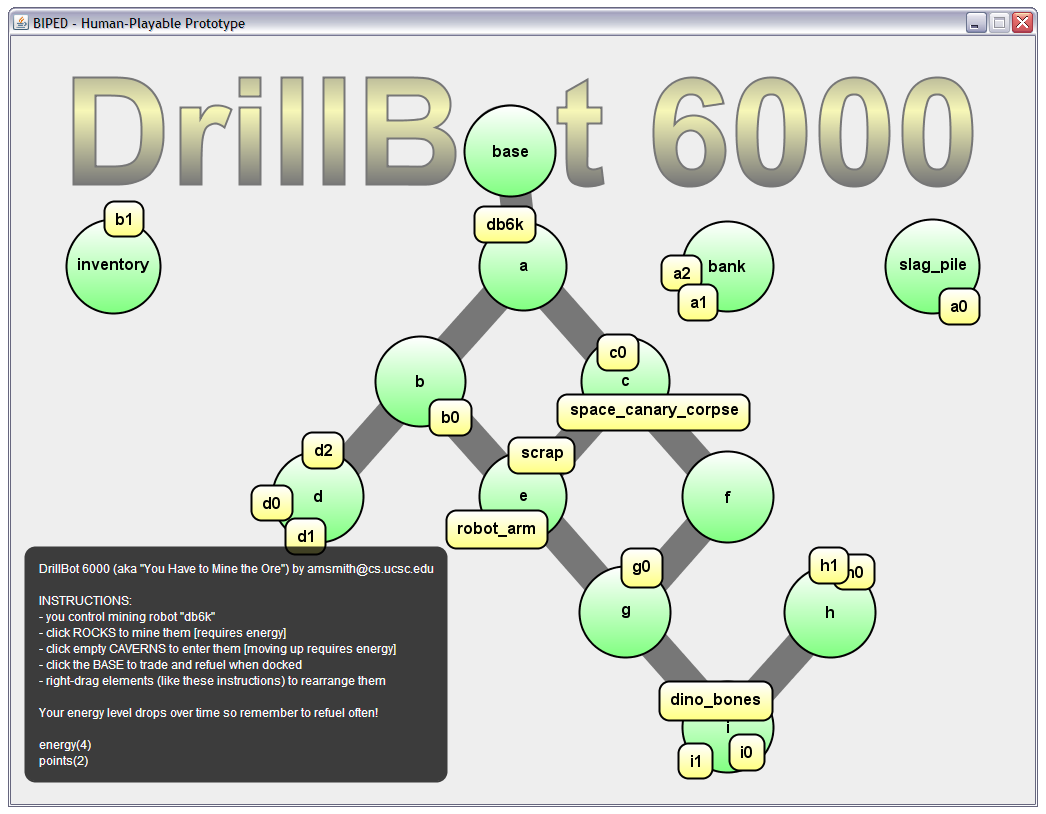
\includegraphics[width=\columnwidth]{db6k_screenshot.png}
\caption{Example of a playable version of a game specified in \ludocore, within
a game engine based on paper-prototyping-style graphical elements. An
automatically generated gameplay trace for this game is shown in
Figure~\ref{fig:trace}.}
\label{fig:biped}
\end{figure}

An existing way to represent purely abstract games in logic is GDL, the game
description language~\citep{GDL}. GDL was designed to specify games for the
general gameplaying competition~\citep{GGP}, in which computers competitively
play unfamiliar, turn-based games. Thus, the language itself was designed
primarily to write infrequently-edited specifications to be read and understood
by computer players as state-transition systems. In contrast, when modeling
videogames, designers are much more concerned with the ease with which they can
incrementally build up a game's rule system through a series of
experimental tweaks~\citep[p.\ 14]{Fullerton}. \Ludocore{} supports this
kind of modeling, at least for technically savvy designer-programmers.

Our iterative-design motivation also contrasts with the goals of formal
verification. While verification attempts to prove that a set of desired
properties hold, it is not clear during a game's prototyping phase which
properties are even desirable. In fact, coming to understand what properties a
game has, and which ones would be desirable, is the main challenge.

Our bridge from games to formal logic is based on the event calculus, a logical
formalism commonly associated with commonsense reasoning. In previous
research~\citep{AIIDE08}, we proposed that the event calculus is an attractive
basis on which to build informative, queryable prototypes. Since then, in
building games with the event calculus, we encountered various design patterns
and idioms, common to all games; it is this experience which prompted the
design of \ludocore.

\section{Building Games on the Event Calculus}

Standard game-design texts discuss a game's mechanics in terms of objects with
dynamic properties (the state of the game), and triggered behaviors (events and
conditional state updates)~\citep[p.\ 295]{Adams}~\citep[p.\ 112]{Fullerton}.
While state and events can be modeled with several
formalisms, or even ad-hoc logical encodings, a common challenge is the well
known frame problem, commonly solved by adding frame axioms. In a language like
GDL, frame axioms explicitly declare when state doesn't change from turn to
turn.  An alternate proposed solution is based on the commonsense law of
inertia~\citep{Shanahan:inertia}, which reads that states retain their values
until an event changes them. This mirrors the usual game-programming assumption
that variables stay set to the same value until changed by an active behavior.

Given our desire to model state and events, and avoid frame axioms that are
tedious to maintain, the event calculus~(EC) is a natural choice.
Additionally, there is a large body of literature discussing the use of EC as a
practical knowledge representation, \emph{e.g.}\ Mueller's
book~\citep{Mueller:book} on applying it to commonsense reasoning problems
involving interaction of objects over time, for which inertial state is the
common case.

The discrete event calculus~\citep{DEC} is based on fluents (predicates
whose truth values vary over time) and events, which happen at particular
integer-valued timepoints and can change the truth values of fluents. Its key
predicates are: \logical{happens(E,T)}, which says that an event happens at a
timepoint; \logical{holds\_at(F,T)}, which says that a fluent is true at a
timepoint; and \logical{initiates(E,F,T)} and \logical{terminates(E,F,T)}, which
map event occurrences to changes in fluent truth values. In addition to state
that does not change without cause (inertial fluents), the circumscription used
in the event calculus implies that events have no effects besides those that
can be derived. Together, these two kinds of default reasoning give the event
calculus elaboration tolerance~\citep{McCarthy:elaboration}, the ability to
modify a knowledge representation without re-engineering it, because new
assertions override defaults.

To realize EC in a computational setting, we use answer-set programming (ASP),
an approach proposed in unpublished notes accompanying
Mueller's book~\citep{Mueller:book},\footnote{\url{http://decreasoner.sourceforge.net/csr/ecas/}} which
\citet{ECASP} proved preserves the expected EC semantics.  Answer sets are sets
of literals that represent acceptable beliefs in an abstract world~\citep{ASP}.
When applied to programs in the discrete event calculus, these answer sets
amount to assertions about what was true and what happened at each timepoint.
Further, for games modeled in EC, the narrative of events amounts to what we
call a gameplay trace. While there are more direct ways to extract a single
trace from a game, ASP does not forward-simulate a game, but rather reasons
abstractly about the space of possible executions, which is far more flexible.

The combination of EC+ASP is an interesting tool for game-related AI because
ASP provides fast inference to models of a game's execution, and EC is a solid
knowledge representation for abstract worlds. Together they facilitate
generating traces from concise declarative descriptions.  This trace inference
is in fact more expressive than forward-search based methods such as Monte
Carlo rollouts; for example, it can definitively prove certain properties of a
game, rather than simply showing that they are unlikely.

\section{The Logical Game Engine}

There some drawbacks to modeling games directly in EC+ASP. In particular,
nearly all of the $T$ variables are superfluous because, outside of the event
calculus axioms, the logical rules of a game tend to refer only to the current
time. Secondly, crafting more complex games directly in the event
calculus formalism leads to duplication of common preconditions for an event in
each of its initiates/terminates clauses. This duplication creates a
maintenance challenge for the game's author, who might want to make simple
changes to the conditions for a particular event. Finally, expressing the fact
that some set of game events conflict with each other, despite being
independently possible, requires mapping a complex idiom (of threading special
conditions through most game logic) over each new game design. Mutually
conflicting events are a common occurrence even in simple turn-based games,
but describing this constraint directly is, in our experience, error-prone.
These annoyances are resolved in our engine while retaining the advantages
of EC+ASP.

Programming computer games is an immensely difficult task, and only through the
continued application of software engineering practices has a sequence of
increasingly powerful game engines made possible the rich games we expect
today~\citep{Blow:Harder}. Game engines attempt to provide standard solutions
for game programming problems without prescribing particular rules or setting
for a game. These solutions are exposed by a set of APIs that games can be
programmed against. Some engines, such as
Torque\footnote{\url{http://www.torquepowered.com}} and
Unreal,\footnote{\url{http://www.unrealtechnology.com}} go so far as to provide
custom programming languages to ease the integration of a game's specification
with the engine's services. \Ludocore{} is modeled after this richer variant of
game engines: it provides not only APIs that encapsulate solutions to difficult
logical modeling problems (such as conflicting events) but effectively provides
a new language that is tailored to the application of specifying logical game
worlds. Games produced with our engine are not only smaller than their
equivalent specification using only the event calculus, but also easier to maintain
throughout meaningful design changes, and easier for the game's author (or even
automated tools) to analyze.

\begin{figure}
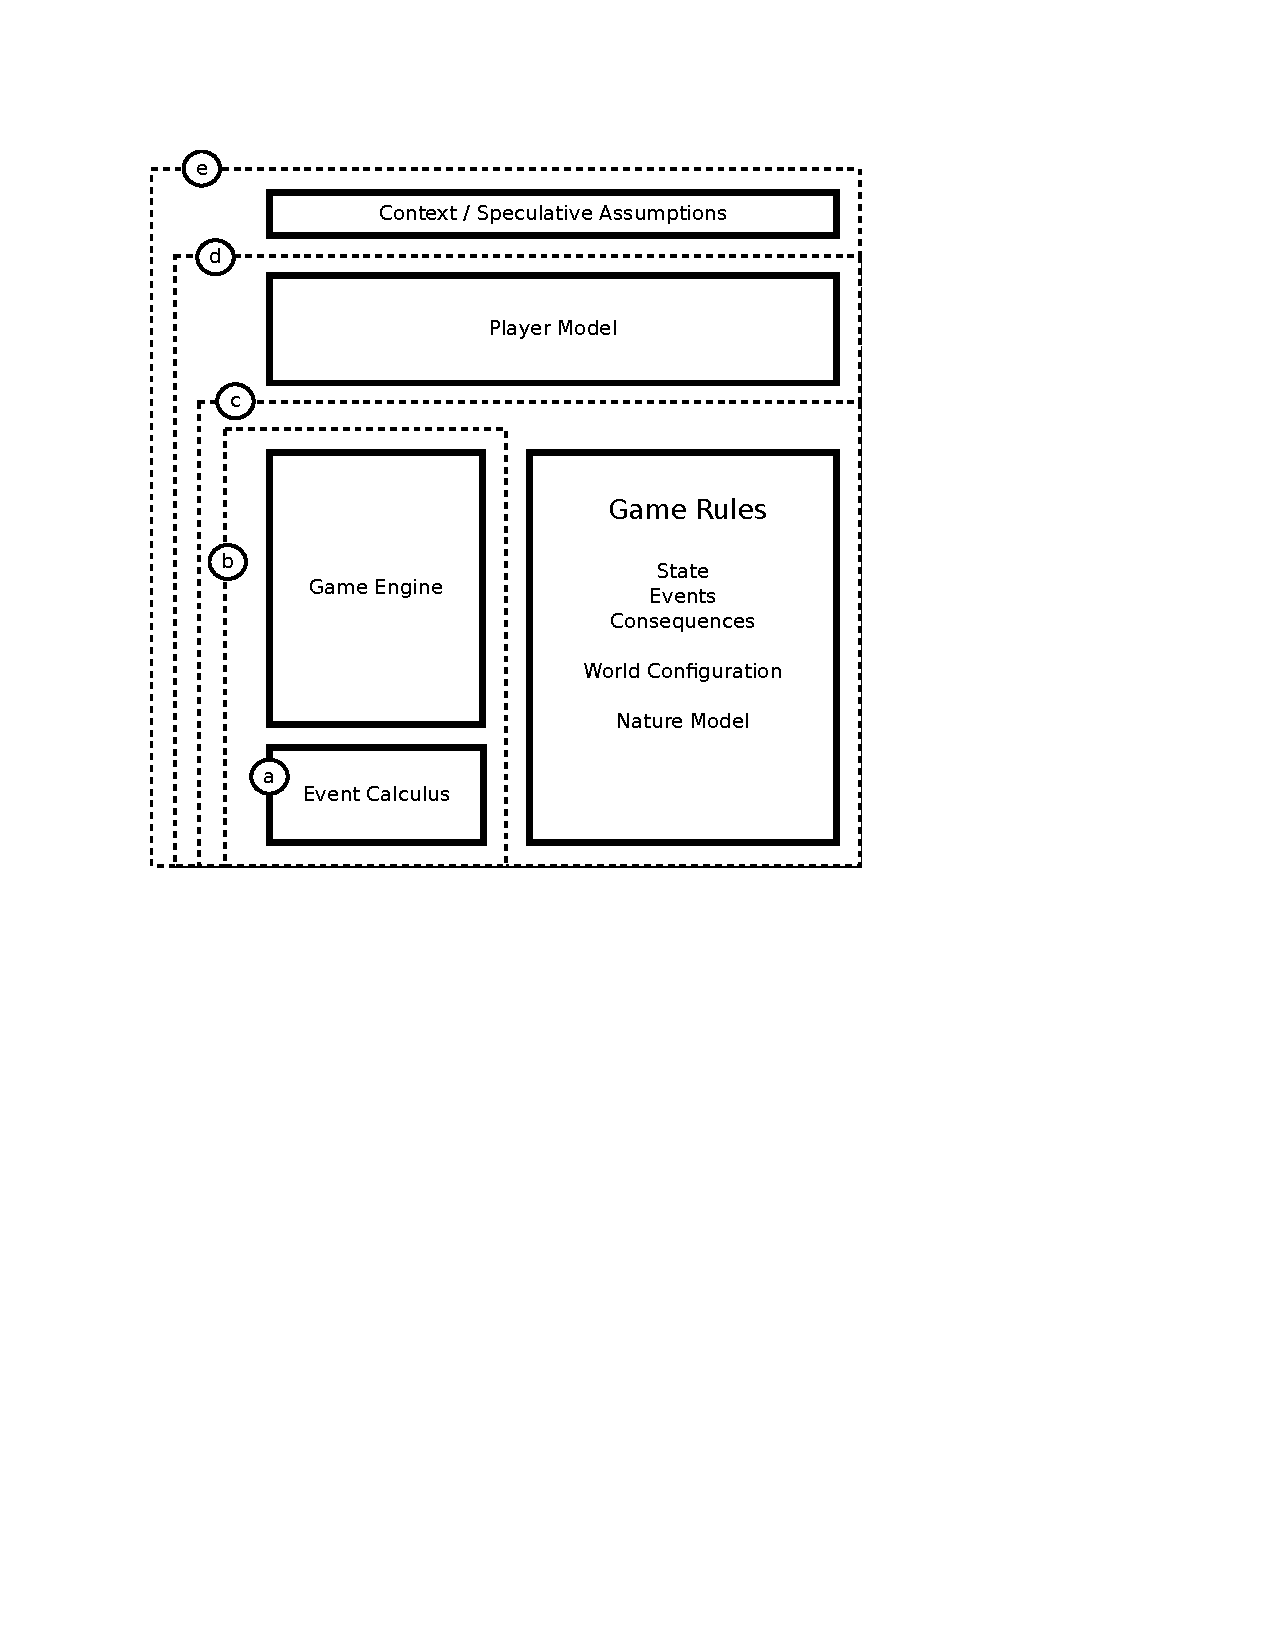
\includegraphics[width=\columnwidth,trim=1in 5.2in 2.7in 1in,clip=true]{ludocore_anatomy.pdf}
\caption{Block diagram illustrating how the logical theories involved in a
complete application of \ludocore{} fit together to form a logic program:
(a) provides a temporal logic basis; (b) expands the temporal logic to include
videogame-level concepts; (c) is a complete specification of a particular game;
(d) provides a model of a certain class of players playing this game; and (e)
represents a focused view of particular situations that could arise in this
player's play.
}
\label{fig:anatomy}
\end{figure}

Our game engine is essentially a background theory for logical game
descriptions. In the rest of this section we will describe the logical
predicates of our game engine and how individual games can leverage them.
Figure~\ref{fig:anatomy} gives an overview of how our engine builds on the
event calculus, and in turn supports modeling games on top of it.
The event calculus axioms provide the base semantics for discussing state
and events over time. Our engine adds higher-level abstractions for modeling
games than the raw event calculus primitives do (discussed below).

To produce a completely specified logical game that admits automatic gameplay
trace generation, the author adds a particular game's rules: the specific state
and events that make up the game, the consequences of events happening in the
game world, the configuration of entities within the game world (\emph{e.g.}
level layouts), and a model of when things take place in the game world without
the player's intervention (caused by ``nature''). While this fully specifies a
game world, a player model additionally adds assumptions about what kinds of
actions a player can take, in which combinations---either due to actual
restrictions (\emph{e.g.} if the author has in mind an input
mapping\footnote{We discuss elsewhere~\citep{Nelson:Towards} why, when modeling
games, input mappings make sense to model separately from the mechanics that
define a gameworld.} that would make certain actions impossible to perform
simultaneously), or due to a desire to investigate certain kinds of player
behavior. Finally, speculative assumptions can be added that restrict the
generated traces to certain kinds of situations that the author wants to
investigate.

\subsection{State, events, and consequences}

Since state and events are natural elements of a game's definition, we expose
the event calculus's fluents and events in our game engine with the predicates
\logical{game\_state} and \logical{game\_event}, respectively.  A game state
assertion in \ludocore{} looks like this:

\snippet{game\_state(at(A,R)) \leftarrow agent(A), room(R).}

This assertion reads that \logical{at} is conceptually a table that records the
relation between agents and rooms (answering, ``is agent $A$ in room $R$?'').
Elements of this table stay set until changed otherwise, a property inherited
from the event calculus's commonsense law of inertia.

For state that should be updated dynamically as a function of other state, we
provide the \logical{state\_helper} mechanism, which provides a computed view on
inertial state. State helpers are, semantically, event-calculus fluents with
inertia disabled, which cannot be directly initiated or terminated. This
stratification into primary and derived fluents that we enforce syntactically
is one safe idiom for avoiding the ramification problem in the event
calculus~\citep{Shanahan:ramification}.

The \logical{state\_helper} assertion below provides a convenient view on the
\logical{at} state for checking when a particular agent is at their starting
location (\logical{starts\_in}) without having to name that location. This
example also illustrates how rules can be conditioned on the current game state
using the \logical{holds} predicate. This state helper rule implies that
\logical{home} is a dynamic (time-varying) property of the game world:

\snippet{&state\_helper(home(A)) \leftarrow\\&\qquad holds(at(A,R)), starts\_in(A,R).}

Game-event declarations are relatively straightforward. The assertion below
describes the event of an agent performing a healing action:

\snippet{&game\_event(heals(A)) \leftarrow agent(A).}

However, game events can have significantly more structure in \ludocore{} than in
the event calculus alone. For example, the conditions under which a game event
is possible (\emph{e.g.}, the legality of moves in a board game) are specified
using the \logical{possible} predicate. In this example, agents may only
heal in their starting room:

\snippet{possible(heals(A)) \leftarrow home(A).}

Possibility assertions are used not only for defining the rules of the game,
but also to control event selection when generating gameplay traces.  Importantly,
possibility is deeply intertwined with the event conflict mechanism.  An
assertion like the one below can keep two otherwise \logical{possible} events
from happening together:

\snippet{conflicts(heals(A), moves(A,R)).}

By providing \logical{possible} and pairwise \logical{conflicts} conditions for
game events in a game model, the required event-selection logic can be
implemented and debugged once in the game engine, instead of by each game
author. By default, actions that are not marked to conflict are safe to
co-occur (whereas GDL enforces exactly one player action per turn, which is
unsuitable for modeling general videogames).

Game events can be tagged by the game's author with whether they are direct
player actions or spontaneous actions that can only be caused by a non-player
entity, thought of as ``nature'' or ``the game master''. The
\logical{player\_event} and \logical{nature\_event} predicates signify this
tagging. Although these annotations do not correspond to what we normally think
of as game rules, they play an important role in scoping the applicability of
player-modeling rules, described with the \logical{player\_asserts} and
\logical{player\_forbids} predicates (and corresponding nature predicates),
discussed later.

Linking game state to game events, the \logical{initiates} and
\logical{terminates} predicates from the event calculus are exposed to game
authors with minimal change. The only modification our engine uses is that
these predicates are defined in a time-invariant fashion, always referring to
the current game state. The example below asserts that the \logical{moves}
event causes an update to the \logical{at} game state, and that the \logical{hits}
event causes the target of the hit to no longer be \logical{alive}, under
certain conditions:

\snippet{&initiates(moves(A,R), at(A,R)).\\
&terminates(hits(A_1,A_2), alive(A_2)) \leftarrow\\&\qquad holds(armed(A_1)), not\ holds(armed(A_2)).}

Finally, the initial state of the game world is given by, simply enough, the
\logical{initially} predicate, which is often conditioned on world
configuration. Even in the examples above, we have suggested the existence of
\logical{room} and \logical{starts\_in} predicates as background knowledge
used to control our state-and-event logic. Many predicates of this kind can be
thought of as specifying a static world configuration: time-invariant facts
about the game world, such as level geometry, item properties, and tables of
weapon effects.

\subsection{Player model interface}

In addition to tagging the subset of game events that are player actions with
\logical{player\_event}, we build an additional interface for specifying models
for players' behavior.

Simply allowing a certain set of events to be considered by the player,
by tagging them as player events, does not immediately yield an expressive
modeling interface. The \logical{player\_asserts} and \logical{player\_forbids}
predicates can be used to express stronger preferences that an action be taken
or should never be taken under any circumstances (\logical{forbids} beats
\logical{asserts} in our engine). The example below illustrates these assertions
in the context of a hypothetical game in which picking up objects is a player
action:

\snippet{&player\_asserts(pickup(O)) \leftarrow kind(O,gold).\\
&player\_forbids(pickup(O_1)) \leftarrow\\&\qquad kind(O_1,K), holds(carrying(O_2)), kind(O_2,K).}

This model describes a player who never misses a chance to pick up a gold
object, but never picks up duplicates (even of gold objects).

The combination of such assertions allows for the specification of a complex,
nondeterministic player action policy that automatically respects the game's
mechanics. The default player model is maximally permissive (it reads that the
player considers all player events) which allows meaningful play traces to be
extracted from games even when no effort has been put into player modeling.
Every clause of \logical{player\_forbids} or \logical{player\_asserts} serves to
pare down the space of gameplay traces to those that are more reasonable to expect,
given the provided knowledge.

Identical in structure to the player modeling interface, we provide
\logical{nature\_asserts} and \logical{nature\_forbids} predicates to operate on
the events marked with \logical{nature\_event}. Whether the nature model is used
to model an opponent, a game master, a collection of non-player characters, or
even used at all, is largely a game author's choice. Many of the rules
that end up in a nature model could be pushed into the game's core rules,
resulting in an equivalent logical model. Leaving certain elements of the game
in the realm of the nature model, however, makes it easy to experiment with
modification to these policies without modifying the accepted base rules. Having
such flexibility is crucial when modeling videogames with a live world, full
of enemies, moving platforms, and other active, non-player entities.

\subsection{Relation to the general event calculus}

In comparison to the general event calculus, we disallow \logical{holds} and
\logical{happens} from ever being used at the head of a rule. In event-calculus
terms, that means we disallow state constraints and triggers.

In general, state constraints are not game mechanics. For example, the state
constraint that the hero is never at the bottom of a pit while alive might be
true of a bit of design, but it is not itself a game rule. There may be rules that
produce this state constraint: for example, saying that the hero dies when he
hits the bottom of pits (a \logical{terminates} clause); and so would a rule
that prevented the hero from ever falling off ledges into pits (a
\logical{possible} clause). The result is that every state is either
only changed by \logical{initiates} and \logical{terminates}, or is known
to be completely passive, in the case of state helpers. Disallowing general
state constraints ensures that games have well-defined, consistent, procedural
meanings (which is required for them to be human-playable).

By disallowing a game's author from directly specifying when an event
\logical{happens}, we can ensure that our engine has complete control over
event management, allowing us to implement \logical{possible},
\logical{conflicts}, and the player and nature models. The logic required to
implement the required semantics of these predicates is highly circular and
counterintuitive. Since such a mechanism is required for almost any interesting
videogame model, by implementing it once and for all in \ludocore, a game
author doesn't have to create an ad-hoc reimplementation of similar constructs
for each game they model.

While we disable rules with \logical{happens} at the head, our engine permits a
conceptual equivalent to the use of triggers (rules that specify that an event
happens whenever a particular combination of state holds) through the nature
model. For example, to model a triggered collision event, the nature model
could include a line that says \logical{nature\_asserts} the collision event
between two objects if their position is identical.

In summary, our engine provides a modified view of the event calculus that
is designed to make game-level assertions easy to express while minimizing the
possibility of a game author (modeler) accidentally introducing purely logical
bugs such as deductive loops and contradictions.  This lets designers focus on
whether their set of game rules is an interesting game, and how it functions,
as opposed to spending much time worrying about whether their set of logical
assertions specifies a game at all. It should be clear from
Figure~\ref{fig:anatomy} that a complete, inspectable model of play includes
much more than just the event calculus.

\section{\Ludocore{} in Action}

Having defined the major ideas in our game engine, we now use it to
generate interesting gameplay traces, and to perform incremental rule
modification, world configuration changes, and player modeling.

\subsection{Gameplay Trace Inference}

The simplest use of our engine is to simply generate any gameplay trace
compatible with a game's definition. One of the difficulties for game designers
is understanding the potential consequences of rule interactions. When
initially crafting game models, these unconstrained traces provide quick access
to possible interactions within the game, quickly revealing undesirable
behaviors resulting from game-design bugs.  The output of our tools provides
not only a log of game events, but the complete game state at all times, to
ease diagnosis.

Figure~\ref{fig:trace} shows an automatically generated event trace from the
\ludocore{} model of a popular online game,
\emph{Motherload},\footnote{\url{http://www.xgenstudios.com/play/motherload}}
in which a mining robot recovers ore and treasures from a network of caverns
without running out of fuel (our playable model of the game is illustrated in
Figure~\ref{fig:biped}). In this case, we show both player-action events, such
as \emph{mine(a1)} (the player's robot mined the rock named \emph{a1}, which
removed it from the world and added it to the robot's inventory), and natural
events, such as \emph{drain} (the robot's energy drains by one unit). The player
here mines a single rock reachable from the starting location, and trades it in
and refuels. Then, he embarks on a longer mining journey, mining a few rocks and
moving downwards into the ground, before finishing with some fairly aimless
wandering up and down.  The values of each piece of game state at each time
step can also be viewed, but we focus here on just the event trace.

\begin{figure}
%\begin{Verbatim}[frame=single,fontsize=\scriptsize]
\parbox{\columnwidth}{\tt
\begin{tabular}{rll}
happens(&\textbf{mine(a1)},&0).\\
happens(&\textbf{drain},&1).\\
happens(&\textbf{drain},&2).\\
happens(&\textbf{trade},&3).\\
happens(&\textbf{refuel},&3).\\
happens(&\textbf{mine(a2)},&4).\\
happens(&\textbf{mine(a0)},&5).\\
happens(&\textbf{down\_to(a)},&6).\\
happens(&\textbf{mine(space\_canary\_corpse)},&7).\\
happens(&\textbf{mine(c0)},&8).\\
happens(&\textbf{down\_to(c)},&9).\\
happens(&\textbf{down\_to(f)},&10).\\
happens(&\textbf{up\_to(c)},&11).\\
happens(&\textbf{up\_to(a)},&12).\\
happens(&\textbf{down\_to(c)},&13).\\
happens(&\textbf{down\_to(f)},&14).
\end{tabular}}
%\end{Verbatim}
\caption{Example gameplay trace for the game shown in Figure~\ref{fig:biped},
generated by asking our analysis engine for a random 15-time-step trace with no
constraints.}
\label{fig:trace}
\end{figure}

While Figure~\ref{fig:trace} shows a random trace with no constraints, the most
common use of \ludocore{} is combining a game with a set of hypothetical or
speculative assumptions (SAs). SAs are commonly used to assert that certain
events do happen or never happen, or that a certain condition is met by a
certain timepoint (\emph{e.g.}, victory within 20 turns). This helps explore
the space in a much more focused way than simply looking at random gameplay
traces; for example, while the random wandering up and down in
Figure~\ref{fig:trace} is a common feature of random traces, it doesn't
illustrate anything particularly interesting about the gameplay possibilities.

The mechanism of specifying speculative assumptions (based on integrity
constraints) provides a simple, modular querying interface for narrowing down
to more interesting traces, and asking questions about gameplay possibilities.
``Is my game winnable?'' requires only one SA to specify (asserting that
\emph{victory} happens at some timepoint). To scope the question further,
asking ``is my game winnable with avatar health never dropping below 5?'',
requires only one more SA. In our model of \emph{Motherload}, we used SAs to
look at extreme kinds of gameplay possibilities: speed runs by players beating
the game in as short a time as possible, or what kinds of gameplay would result
if a player never refuelled, or refuelled cautiously. We compared these traces
to traces from human playtesters, who gave us an idea of how beginners would
play the game before being familiar with it, which showed us, for example, that
our players were \emph{much} more cautious on refuelling than
necessary.\footnote{We discuss this complementary use of human and machine
playtesting in more detail elsewhere~\citep{AIIDE09}.}

In generating these kinds of constrained traces, the logical inference approach
taken in EC+ASP shines. Had we used randomized forward search in the game's
state space, constraints on happenings of the final timepoint would be
difficult to encode and inefficient to compute, requiring exhaustive search to
prove nonexistence.  ASP lets us ``run the game backwards'' or even
sideways\footnote{Inferring which state is compatible with a particular
narrative of events} as needed to satisfy trace constraints or quickly prove
them impossible.

While gameplay traces can be highly informative (because each includes a
complete narrative of events), even the absence of traces can be informative.
If adding a particular SA yields no traces for a game that previously admitted
many, then it has been proven (by contradiction) that the SA is incompatible
with the game's rules, \emph{i.e.}\ that the assumption is false in the game's abstract
world.\footnote{\citet{Thielscher:singleplayer} also uses termination without
models of an ASP solver to prove properties of a game via contradiction.}

Extraction of gameplay traces is the primary function of the \ludocore{}
engine. The affordances we describe below for modeling and modifying games all
serve to give the game's author the ability to sculpt the space of traces that
our system will generate.

\subsection{Modifying rules and configuration}

Recall that game design is often an iterative process, adding, removing, and
tweaking rules as a design progresses. Rules, in \ludocore, are represented by
the \logical{game\_event}, \logical{game\_state}, \logical{possible},
\logical{conflicts}, and \logical{initiates}/\logical{terminates} predicates. A
game's author might make changes to these rules (and examine the traces for the
new game) as part of a major intentional design change, or simply as a way of
quickly testing the implications of alternative formulations of a particular
mechanic in the game. Often it is useful to disable (by simply commenting-out)
several rules to focus on sub-parts of a game in isolation without distracting
interactions, \emph{e.g.}\ disabling ammunition consumption on weapons when
examining health-point management. In a language without elaboration tolerance,
this would require more complex editing than simply commenting out a rule. Creating
a variant of chess without castling in GDL, for example, cannot be done simply
by removing the castling rule, but requires other edits as well.

To illustrate rule modifications, we draw on two examples from our \ludocore{}
model of \emph{Motherload} (discussed earlier, and shown in
Figure~\ref{fig:biped}).

If we wanted to add a fixed inventory capacity to our mining robot
(constraining an existing event on the basis of existing game state), we would
modify the \logical{possible} conditions for our game's \logical{mine} event to
depend on a count of the number of items for which the \logical{bagged} state
for rocks held. This single change would not only stop traces that violate the
new rule from being generated but reject traces when even an externally assumed
narrative included too many mining events:

\snippet{&state\_helper(have\_space) \leftarrow\\&\qquad count(R,holds(bagged(R)),N), N<10.\\
&possible(mine(R)) \leftarrow\\&\qquad holds(present(R)), touching(R), fueled, have\_space.}

To modify the game to charge players energy points for mining instead of
moving, we would drop the \logical{initiates} and \logical{terminates} rules
linking the moving event to the energy state and create two new ones linking
mining to moving (one to terminate the previous energy value and another to
initiate the diminished value). This re-wiring task incurs only a four-line
change to the game source when using our engine, due to the conciseness of
expressions enabled by our game engine.  With access to gameplay trace
inference, we can quickly verify the effectiveness of the rule modification
without the need for human play testers.

This ease of rule modifications directly derives from the elaboration tolerance
afforded by the underlying EC formalism.  \citet{McCarthy:elaboration}
describes elaboration tolerance as the ability (of a knowledge representation)
to accept changes to known facts without having to ``start over'', which is exactly
what we realize for the space of games. Further, in other research applying EC
to games, we have shown how entire modules (corresponding to game mechanics and
vocabularies) can be swapped in and out without trouble~\citep{AIIDE08}.

In addition to swapping rules, it is quite easy to pair a fixed game with
different sets of configuration such as map layout, static item properties, and
tweakable constants.  For example, a simple map can be used for early testing,
and a more complex one used later for detailed player modeling.  In addition to
manually specified game configurations, it is possible to let the ASP solver
reason across possible configurations for the game. In our model of the game
\emph{Minesweeper}, we are able to reason over possible placements of mines
that are consistent with player observations. In a simple dungeon crawl game,
we allowed the solver to manipulate the presence and connectivity of rooms on a
map. The ability to make structural queries of this sort is a novel feature for
game engines.

\subsection{Using player and nature models}

While we think of speculative assumptions as convenient but throwaway
constraints, specifying complex assumptions can be tedious. The player modeling
interface provides a more straightforward way of building larger player models
that will be retained and modified, rather than used in only a few queries.
Sets of \logical{player\_asserts} and \logical{player\_forbids} clauses are
collected to carve out the space of behavior that can be reasonably expected of
the kinds of player being investigated.

A custom nature model can similarly be used to carve the behavior of other in-game
entities. In the dungeon crawl game, we used the nature model to control
monster wandering behavior. We had tagged the monster movement event as a
nature event, implying that it should always be considered in trace finding
when using the default nature model. To effect patrolling behavior, we used the
following assertion, which yields monsters who wander only within their own
marked areas:

\snippet{&nature\_forbids(move\_to(M,R)) \leftarrow\\&\qquad not\ patrolled\_by(M,R).}

\section{Applications Enabled}

\Ludocore{} enables a number of broader applications, some of which have
already been investigated in other forms.

\subsection{Game design}

Designing games in a logical game engine, or at least using one to prototype
game ideas, can provide designers with insight about design pros and cons, and
suggest possible improvements. Many logical formalisms can allow verification
that desired properties hold, and undesired properties don't. However,
designers often work in an iterative, exploratory manner, and find exact
yes-or-no queries somewhat difficult to formulate~\citep{FDG09}.
The experimentation with gameplay traces that our engine supports can help
designers understand the possibilities of their design by iteratively ``zooming
in'' on specific kinds of traces using SAs, and observing how different player
models shape emergent properties of the game. We have already begun pursuing
this application, creating a game prototyping system~\citep{AIIDE09} in which
human-playable, board-game-like prototypes can be built, using the logical
representations described in this paper.
Figure~\ref{fig:biped} shows an example designed as if to be an early
prototype version of \emph{Motherload} (discussed earlier).  This prototype
focuses on the core mechanics: moving around underground, mining, and refueling
(whereas \emph{Motherload} also includes shopping for upgrades and story
elements).  These prototypes support two kinds of playtesting: traditional
observations of human players, and a new mode of machine playtesting, in which
observation of machine-generated gameplay traces is the focus.

Logical game engines may also form a core component of emerging research in
automated videogame design. In a non-logical approach,
\citet{Togelius:Experiment} generate \emph{Pac-Man} variants from a
parameterized space and use reinforcement learning to demonstrate gameplay in
the resulting games. Games implemented in \ludocore{} can be varied in a much
more open-ended and incremental manner than with a parameterized space of
variation, and its elaboration tolerance addresses the problem of brittleness
of symbolic representations, which was in part responsible for the move towards
parameterized numerical representations in content-generation research.

Furthermore, given sets of traces, inductive logic programming~(ILP) can be
used to induce models for the style of gameplay exhibited in those traces. The
player modeling interface in \ludocore{} makes this more feasible by
having player models built from only two key predicates. Many popular ILP
systems, such as Progol~\citep{Progol} can only learn single predicates at a
time. In our player modeling interface, single-predicate ILP systems can learn
the \logical{player\_asserts} predicate from example gameplay traces. Some research has
even been done on learning EC rules themselves~\citep{ECILP}, which, for games,
would open up the possibility of inducing new game rules from a collection of
desired gameplay traces.

Procedural level design can be done by specifying and solving constraints for
what constitutes a good level, sometimes as part of a larger search
process~\cite[e.g.][]{Gillian:FDG09}. Particularly relevant here, a
community-driven project recently added procedurally generated maps and base
layouts to the real-time strategy game \emph{Warzone 2100}, using ASP to specify and
solve constraints on the maps'
layouts.\footnote{\url{http://warzone2100.org.uk/manual-diorama}} Designing a good level,
however, often means designing a level that supports good gameplay, and these
sorts of static constraints only indirectly speak to gameplay. Other
approaches, such as that of \citet{Togelius:levels},
generate levels and score them with a fitness function that predicts whether
they support interesting gameplay. For games written using our logical game
engine, a constraint-based approach can easily include these kinds of
constraints on gameplay in addition to constraints on static level properties,
because the level-generation search and game-tree search are unified into the
same query mechanism. 

\subsection{Crafting game playing agents}

Despite our motivating focus on analyzing game designs, our logical game engine
has applications to playing games as well. Because gameplay trace inference in
our engine corresponds exactly to what is commonly known as EC
planning~\citep{ECplanning}, it is possible to use our engine directly in a
general game player. \citet{Thielscher:singleplayer} already argued for the
applicability of ASP with temporal-logic models for the contemplation phase of
GGP competitions.

The player modeling interface we provide is designed to accept incremental
additions of knowledge about how a player (or their opponents) make choices.
Though this interface cannot express a minimax-like policy (that includes
quantification over models at every timepoint), it does coalesce facts into a
unified move-set selection policy which would allow minimax to operate in the
more restricted space in which the modeled opponent is really playing.

The ease of adding and removing rules in our games has another benefit for
those wishing to craft general game players. The elaboration tolerance of the
representation makes syntactic construction of novel games much easier. By
building all combinations of a fixed set of add-on mechanics, a generative
space of games can be realized, providing a much wider selections of games for
agents to be tested on. 

\section{Conclusion}

In this paper, we introduce a new concept: the logical game engine. Our logical
game engine, \ludocore, much like a traditional game engine, both provides a
higher-level language to describe games, and centralized solutions to tedious
or error-prone programming tasks. By virtue of using logic, we gain not only a
concise representation of a game's mechanics, but also the ability to
automatically generate interesting gameplay traces that meet meaningful
constraints.

While clearly \ludocore{} serves as a bridge from the concerns of game design to
logic-based AI tools, it has also served as the basis for implementing
interactive prototypes. In BIPED~\citep{AIIDE09}, human-playtestable
prototypes with real-time interaction and graphics are written with the
\ludocore{} engine, enabling the same game specifications to both be used with
logical tools (objective, machine playtesting) and as gameplay demos
(subjective, human playtesting).

Apart from demonstrating its utility by building BIPED on it, the question of
how to evaluate \ludocore{} itself is more subtle. We are not immediately
interested in metrics such as benchmarks. Rather, the primary driver of our
research is expressiveness, the ability for human or automated game designers
to succinctly specify and informatively query models of gameplay. We want to
answer questions such as: How easy is it to specify different kinds of games?
Is making common kinds of modifications to a game easy? Are there queries we
can't answer from this kind of model? We've designed with these questions in
mind, but a satisfying answer to these questions must come from the kind of
extensive case studies that look at the evolution of a multiple game designs
through many stages of modification.

Future work on \ludocore{} will aim to further improve the process of
specifying, working with, and reusing formal game models. Although the event
calculus' elaboration tolerance gives specifications some built-in modularity,
a higher-level module system would make it easier to quickly swap in and out
larger subsystems, such as pre-specified inventory systems or economy models.
Language improvements can also simplify the specification of many common kinds
of game mechanics, for example by adding inheritance between game objects, or
higher-level handling of numerical operations.  Finally, our goal in building
\ludocore{} is to enable two main applications: an automated game design system
that can understand and manipulate game rules~\citep{VF}, and a game-design
prototyping system that provide designers quick feedback and deeper insight
into early-stage designs~\citep{FDG09}. 

\bibliographystyle{IEEEtranN}
\bibliography{references}

\end{document}
